\documentclass[UTF8,a4paper,zihao=-4]{ctexart}

\usepackage[
  left=2.5cm,right=2.5cm,
  top=2.6cm,bottom=2.6cm,
  headheight=15pt,headsep=22pt,footskip=30pt
]{geometry}
\usepackage{amsmath,amssymb}
\usepackage{booktabs,longtable,tabularx,array,multirow}
\usepackage{graphicx,float}
\usepackage{xcolor}
\usepackage{tikz}
\usetikzlibrary{arrows.meta,positioning,shapes.geometric}
\usepackage{enumitem}
\usepackage{fancyhdr}
\usepackage{hyperref}

\definecolor{accent}{HTML}{176B87}
\definecolor{softblue}{HTML}{EAF4F8}
\definecolor{softgray}{HTML}{F3F4F6}
\hypersetup{colorlinks=true,linkcolor=accent,citecolor=accent,urlcolor=accent,pdfauthor={匿名参赛团队},pdftitle={声速测量虚拟实验教学资源设计报告}}
\setlength{\parindent}{2em}
\setlength{\parskip}{0.25em}
\setlist{nosep,leftmargin=2em}
\renewcommand{\arraystretch}{1.25}
\pagestyle{fancy}
\fancyhf{}
\fancyhead[L]{第十二届全国大学生物理实验竞赛（创新）}
\fancyhead[R]{自选题2：教学资源和虚仿}
\fancyfoot[C]{\thepage}

\newcommand{\code}[1]{\texttt{#1}}

\begin{document}

\hypersetup{pageanchor=false}
\begin{titlepage}
\thispagestyle{empty}
  \centering
  \vspace*{1.5cm}
  {\zihao{2}\bfseries 第十二届全国大学生物理实验竞赛（创新）\par}
  \vspace{0.8cm}
  {\zihao{3}\bfseries 自选题2：教学资源和虚仿\par}
  \vspace{1.8cm}
  {\zihao{1}\bfseries 声速测量虚拟实验室\par}
  \vspace{0.4cm}
  {\zihao{3}回声、时间差、相位与驻波的多方法交互教学资源\par}
  \vfill
  \begin{tabular}{rl}
    作品类别：& 自选题2——教学资源和虚仿\\
    作品形态：& 交互式虚拟实验与智能助教\\
    \multicolumn{2}{c}{日期：\quad 2026年8月}
  \end{tabular}
  \vfill
  {\small 本报告不出现学校名称、指导教师姓名和学生姓名。成员以匿名编号表示。}
\end{titlepage}
\hypersetup{pageanchor=true}

\pagenumbering{Roman}
\section*{摘要}
\begin{sloppypar}
声速测量包含时间、相位和空间波长三类观测思想。传统教学常把不同实验分散讲授，学生容易机械套用公式，却难以理解观测量、信号处理、误差来源和适用条件之间的联系。本作品开发了声速测量交互式虚拟实验室，在同一理论声速与统一交互框架下实现回声法、双麦克风时间差法、示波器相位差法和驻波法。系统同步显示声波的空间传播、原始/含噪信号、自动分析结果和误差读数，使学习者能够调节距离、频率、采样率、信噪比、反射系数、入射角和相位整周期数，比较四种方法的定量结果与局限。

作品还集成本地文献检索和智能问答，用于解释实验原理、图像和误差；确定性物理模型独立计算所有仿真数据，生成式人工智能不修改实验结果。系统采用 Python--Julia 混合编程：Python/Streamlit 承担统一网页、知识检索、问答、安全执行和进程调度，Julia/WGLMakie 承担四种测量模型及浏览器交互图形；两端通过本机回环网页服务协同。作品已封装为 Windows 单文件版本，目标计算机无需预装 Python 和 Julia，便于课堂演示、学生预习和自主探究。报告给出物理模型、数值算法、软件流程、参数范围、结果验证、教学评价方案、运行配置、局限性以及第三方依赖与自研代码边界。
\end{sloppypar}

\noindent\textbf{关键词：}声速测量；时间差；互相关；相位差；驻波；Python--Julia 混合编程；智能助教

\clearpage
\tableofcontents
\clearpage
\pagenumbering{arabic}

\section{选题意义与目标定位}

\subsection{教学背景与选题价值}
声速测量是大学物理实验中连接机械波理论、传感器测量、示波器使用和数据处理的综合性课题\cite{rayleigh1877,morse1948,crawford1968}。基本关系 $v=s/t=f\lambda$ 虽然简洁，但真正的实验任务并不是套用公式，而是判断“测量了哪一段距离、从信号中提取了哪个时间或相位、该观测量在什么条件下能够代表传播过程”。回声法、双麦克风时间差法、相位差法和驻波法分别从传播时间、相关时延、相位和空间周期出发，提供了同一物理量的四种独立观测路径\cite{berg2011,carvalho2007,water2020,standing2024}，适合用于培养多方案测量和交叉验证意识。

实体声速实验能够训练装置搭建、传感器对准和示波器调节；基于声卡、智能手机与简易声管的研究还说明低成本设备能够拓展课外实验场景\cite{carvalho2007,staacks2018,hellesund2018}。但环境噪声、反射面质量、麦克风一致性、房间边界和课堂时长会限制变量探索。学生通常只能完成规定步骤，很难在同一次实验中系统改变采样率、信噪比、距离、入射角、反射系数和相位整周期数，更难把四种方法放在相同声速条件下横向比较。虚拟实验可以保存共同的理论基准，受控地加入非理想因素，展示不可直接观察的传播过程和分析算法，从而帮助学生把“仪器读数”还原为“物理模型—信号—估计量”的完整链条。

本作品以统一真实声速为主线，将四种经典方法组织在同一界面和同一评价框架中。学习者既能研究单一方法，也能比较时间分辨率、相位多值性、空间分辨率和抗噪性能。作品尤其强调方法适用条件：仿真结果不是为了给出一个看似精确的数值，而是为了说明为什么不同观测路径会产生不同误差，以及怎样通过改变实验设计提高可信度。

四种方法还构成了一条由直接到间接的测量认识路径。回声法从最直观的往返时间开始，双麦克风法进一步引入同步采样和信号相关，相位法展示高灵敏度测量中的整周二义性，驻波法则把时间问题转化为空间周期问题。学习者在比较中会发现，同一个 $v$ 可以由不同中间量得到，而每一种中间量都伴随特定的分辨率、系统误差和实验条件。这比孤立完成四次公式代入更能体现物理实验的方案设计思想。

\subsection{现有教学中的主要困难}
空气中声速测量的基本关系看似简单，但四种方法的直接观测量并不相同。若只展示最终公式，学生容易忽略距离定义、同步采样、相位包裹和边界条件。主要困难与作品响应见表~\ref{tab:sound-problems}。

从测量链条看，声速并不是传感器直接输出的量。传感器获得电压随时间变化的离散记录，程序再从峰值、互相关、相位投影或空间极值中提取中间量，最后才能结合几何距离和频率计算声速。若界面只显示最终数值，学生既无法判断异常结果发生在哪个环节，也难以理解算法参数为何会影响测量值。因此作品必须让“传播对象—原始信号—分析量—速度估计”同时可见。

从实验评价看，四种方法并不存在脱离条件的绝对优劣。较长传播距离可能减小时间分辨率造成的相对误差，却会降低信噪比；提高频率可以缩短波长，却可能增加相位整周期判断难度。作品因此不仅要验证公式，还要提供可控的冲突条件，让学生依据证据选择方法、权衡参数并说明结论的适用范围。

\begin{table}[!htb]
\centering
\caption{教学困难与作品设计响应}
\label{tab:sound-problems}
\begin{tabularx}{\textwidth}{p{3.2cm}X X}
\toprule
教学困难 & 典型表现 & 作品设计响应\\
\midrule
距离定义混淆 & 回声往返路程忘记乘 2，或把双麦克风间距误作往返距离 & 空间传播图同步标注声源、反射面/麦克风与有效传播距离\\
读数与算法脱节 & 只接受程序给出的时间差，不理解峰值或互相关的获得过程 & 同时显示原始信号、分析曲线、候选峰和最终估计量\\
忽略采样限制 & 认为增加小数位即可无限提高时间差法精度 & 可调采样率，并展示一个采样间隔对应的速度量化效应\\
相位多值性不清 & 忽略 $2\pi$ 包裹和整周期数，得到数值合理但物理错误的结果 & 显式设置整周期数并比较不同分支对应的传播距离\\
理想驻波等同实测 & 不考虑反射不完全、波节不为零和波节定位误差 & 可调反射系数，显示入射波、反射波、合成波及包络\\
方法彼此割裂 & 能分别套公式，却不能说明各方法的优缺点和适用范围 & 在统一声速与参数框架下比较四种估计值及误差来源\\
\bottomrule
\end{tabularx}
\end{table}

本作品把空间传播、测量信号、分析过程和结果读数同步呈现，并鼓励学习者先预测、再改变单个参数、最后导出数据复算。其目标不是替代实体装置，而是降低理解不可见传播过程和信号处理步骤的门槛。

为帮助学生定位错误，界面把一次测量拆分为四层证据：空间图回答声波实际经过哪段路程，原始波形回答传感器记录了什么，分析图回答算法如何从波形提取时间或相位，结果区回答这些观测量如何进入声速公式。只有四层彼此一致，最终数值才具有可解释性。若估计值异常，学生可以逐层检查距离、信号、算法峰值和单位，而不是把程序输出简单判定为“对”或“错”。

\subsection{作品定位}
作品按“自选题2：教学资源和虚仿”申报，而非实体仪器制作或“AI+物理实验”命题类作品。核心定位如下：
\begin{enumerate}
  \item 自主构建四种声速测量的基本物理模型与数值信号；
  \item 允许调节参数并可视化输出传播、波形、互相关、相位和驻波结果；
  \item 强调测量过程、误差和方法比较，而非直接生成最终答案；
  \item 用智能问答辅助文献学习和实验解释，但保持仿真数据可复算、可追溯；
  \item 通过单文件发布降低安装与维护门槛。
\end{enumerate}

作品遵循三项设计原则。第一是\textbf{同一基准、不同观测}：四种方法共享同一理论声速，使方法差异能够归因于观测机制和参数条件。第二是\textbf{过程透明、结果可复算}：显示信号生成、分析曲线和中间量，并允许导出数据独立计算。第三是\textbf{理想模型与非理想因素分层}：先建立传播时间、相位和波长关系，再逐步加入噪声、采样、角度和反射效应。智能问答用于解释文献和实验图像，不参与产生四种方法的仿真测量值。

上述原则落实为三条相互隔离的数据链。Julia 数值链依据真实声速和参数生成信号、分析量与估计值；网页交互链负责状态显示、动画和数据导出；智能问答链负责检索声学资料、解释方法并调用确定性复算工具。问答模块不能写入仿真结果，图形模块也不依赖生成模型才能运行。这样的结构保证即使模型服务不可用，四种实验仍保持完整，也使每个数值都能追溯到明确的计算函数。

\subsection{适用对象与教学场景}
作品主要面向学习过机械波和基本示波器操作的大学低年级学生，也适用于声学专题课程、开放实验和物理竞赛训练。典型教学场景包括：
\begin{itemize}
  \item \textbf{实验前预习：}辨认四种方法的直接观测量，预测距离、频率或采样率变化对结果的影响；
  \item \textbf{课堂演示：}同步播放空间传播和信号形成，解释时间差、相位差和波节间距的来源；
  \item \textbf{实体实验配套：}将真实波形与理想/含噪仿真对照，定位触发、反射、对准和采样问题；
  \item \textbf{方法比较：}在共同声速下设计等精度条件，从准确度、稳定性、设备复杂度和适用距离评价方案；
  \item \textbf{课后探究：}导出数据，自行实现峰值、互相关、相位投影或波节拟合，并与内置读数交叉验证。
\end{itemize}

在不同教学时长下，作品可形成不同任务组合。短时课堂演示可比较回声往返距离和双麦克风单程距离；完整实验课可安排四组学生分别研究一种方法，再用统一表格交流；开放实验可要求学生导入真实数据、选择最合适的分析算法并讨论不确定度。教师还可设置“同一设备条件下怎样提高精度”或“同一精度目标下怎样降低装置复杂度”等决策题，使参数调节服务于实验设计而不是无目的浏览。

\subsection{教学目标}
本作品将教学目标分为知识、能力、科学思维和实验素养四个层次：
\begin{enumerate}
  \item \textbf{知识目标：}理解 $v=s/t=f\lambda$ 在四种实验中的具体形式以及各自成立条件；
  \item \textbf{能力目标：}能够从波形、相关曲线、相位和驻波包络中提取有效观测量，并完成声速计算；
  \item \textbf{科学思维目标：}能够使用控制变量、量纲分析、极限情形和交叉测量判断结果是否合理；
  \item \textbf{实验素养目标：}认识采样、噪声、对准、反射和环境条件对结果的影响，提出可操作的改进方案。
\end{enumerate}

四类目标依次回答“公式是什么”“观测量怎样得到”“结论依赖哪些假设”“真实实验应如何改进”。例如，学生不仅要写出 $v=2d/\Delta t$，还要指出两个峰的识别方法、采样间隔造成的量化误差以及房间混响可能引入的错误回波。教学目标因此与实验过程逐项对应，评价也不能只检查最终声速是否接近标准值。

\subsection{预期学习成果}
完成实验后，学习者应能：
\begin{itemize}
  \item 正确区分回声往返距离和双麦克风单程投影距离；
  \item 理解采样率对时间分辨率和速度估计量化误差的影响；
  \item 解释互相关峰如何给出两路信号时延；
  \item 说明相位包裹及整周期数选择造成的多值性；
  \item 由驻波波节间距推导波长与声速；
  \item 从准确度、稳定性、设备与适用条件比较不同方法。
\end{itemize}

学习成果通过可观察证据进行评价：概念预测题检查距离和观测量定义，程序导出数据检查独立复算能力，参数扫描报告检查误差规律，四方法比较表检查方案评价能力，实体实验对照记录检查模型边界意识。由此形成“提出问题—选择方法—预测信号—获取读数—独立复算—比较改进”的完整探究链路。

\section{物理原理与计算模型}

\subsection{共同物理假设与测量链}
四种方法虽然观察对象不同，但都建立在同一传播模型上：介质均匀、静止、各向同性且在所用频段内近似无色散，声波沿设定方向传播，测量期间声速 $v$ 保持不变，因而
\begin{equation}
 v=f\lambda,\qquad k=\frac{2\pi}{\lambda},\qquad \omega=2\pi f.
 \label{eq:sound-wave}
\end{equation}
程序把真实声速 $v$ 作为“信号发生器”的共同参数，再模拟仪器取得时间差、相位差或波节间距，最后仅用可观测量反演估计值 $\hat v$。这一区分很重要：若反演阶段直接读取设定的 $v$，就不再是测量仿真。结果统一用
\begin{equation}
 \varepsilon_r=\frac{\hat v-v}{v}\times100\%
 \label{eq:sound-relative-error}
\end{equation}
评价，并保留理论值、测得值和中间信号，使学习者能够独立复算。

数值信号采用理想波形与加性高斯噪声的组合。信噪比为 $\mathrm{SNR}_{\mathrm{dB}}$ 时，程序使用幅度比例
\begin{equation}
 \sigma_n=10^{-\mathrm{SNR}_{\mathrm{dB}}/20}
 \label{eq:sound-noise}
\end{equation}
产生零均值噪声；不同通道使用独立噪声序列，同时固定随机种子，使同一组参数的结果可重复。模型默认采集时钟同步、传感器响应一致，并暂不模拟温湿度梯度、空气流动、频率相关衰减、麦克风群延迟和声卡时钟漂移。这些假设给出了清晰的教学基线，也明确了虚拟结果不能直接替代实体标定。

\begin{table}[!htb]
\centering
\caption{四种方法从可观测量到声速的反演关系}
\begin{tabularx}{\textwidth}{p{24mm}X X}
\toprule
方法 & 直接观测量 & 反演关系与主要二义性\\
\midrule
回声法 & 往返脉冲延迟 $\Delta t$ & $\hat v=2d/\Delta t$；须识别正确回波\\
双麦克风法 & 互相关峰时延 $\Delta t$ & $\hat v=d\cos\theta/\Delta t$；受采样量化和角度影响\\
相位差法 & 包裹相位 $\phi_w$ & $\hat v=2\pi fd/(2\pi n+\phi_w)$；须确定整周期数 $n$\\
驻波法 & $q$ 个波节间隔总长 $D_q$ & $\hat v=2fD_q/q$；须正确识别波节或波腹\\
\bottomrule
\end{tabularx}
\end{table}

\subsection{方法一：回声法的往返时间模型}
声源距反射面为 $d$，直达脉冲与一次反射回声的路程差为 $2d$，故
\begin{equation}
 \Delta t=\frac{2d}{v},\qquad \hat v=\frac{2d}{\Delta t_{\mathrm m}}.
 \label{eq:echo-speed}
\end{equation}
程序用宽度为 $\sigma_t$ 的高斯函数
\begin{equation}
 p(t;t_c,\sigma_t)=\exp\!\left[-\frac12\left(\frac{t-t_c}{\sigma_t}\right)^2\right]
\end{equation}
模拟短声脉冲，采样信号为
\begin{equation}
 s(t_i)=p(t_i;t_0,\sigma_t)
 +r\,p\!\left(t_i;t_0+\frac{2d}{v},\sigma_t\right)+n_i,
 \qquad t_i=\frac{i}{f_s},
 \label{eq:echo-signal}
\end{equation}
其中 $r$ 是反射系数。当前实现取 $t_0=2\,\mathrm{ms}$、$\sigma_t=0.28\,\mathrm{ms}$，分别在两个理论中心附近的 $\pm3\sigma_t$ 时间窗中寻找最大值，以模拟“已知直达脉冲和目标回波大致所在区间”时的峰值读数。反射系数主要改变回声信噪比；在理想模型中不改变传播时间，但当 $r$ 很小或噪声很强时，噪声峰可能取代真实回波。回声教学的关键也正是正确识别回波并使用两倍墙面距离\cite{berg2011}。

峰值只能落在采样格点上，故单个峰时刻具有约一个采样间隔 $1/f_s$ 的量化尺度。对式\eqref{eq:echo-speed}作一阶微分，有
\begin{equation}
 \frac{\delta v}{v}\approx \frac{\delta d}{d}-\frac{\delta(\Delta t)}{\Delta t}.
 \label{eq:echo-uncertainty}
\end{equation}
增加反射距离可增大 $\Delta t$、减小相同时间分辨率造成的相对误差，但过大的距离又会降低回声幅度并引入更多反射，这体现了测量范围与信噪比的权衡。

\subsection{方法二：双麦克风时间差与互相关}
设两麦克风基线长度为 $d$，声传播方向与基线夹角为 $\theta$。平面波在基线方向上的有效路程差为
\begin{equation}
 d_{\parallel}=d\cos\theta,\qquad
 \Delta t=\frac{d\cos\theta}{v}.
 \label{eq:dual-delay}
\end{equation}
程序分别生成中心相差式\eqref{eq:dual-delay}的两个高斯脉冲，并为两通道叠加独立噪声。为避免振幅尺度影响延迟判断，对每一个整数滞后 $k$ 计算重叠区间内的归一化互相关
\begin{equation}
 R_{xy}[k]=
 \frac{\sum_i x_i y_{i+k}}
 {\sqrt{\left(\sum_i x_i^2\right)\left(\sum_i y_{i+k}^2\right)}}.
 \label{eq:dual-correlation}
\end{equation}
使 $R_{xy}[k]$ 最大的 $k_{\max}$ 给出 $\Delta t_{\mathrm m}=k_{\max}/f_s$，再由 $\hat v=d\cos\theta/\Delta t_{\mathrm m}$ 反演。声卡和智能手机飞行时间实验表明，同步双通道记录能把极短传播时延转化为可分析的波形位移\cite{carvalho2007,staacks2018}。

当前算法只定位整数采样点，故时延量化约为 $1/f_s$；后续可用相关峰抛物线拟合或频域相位斜率实现亚采样估计。误差的一阶传播为
\begin{equation}
 \frac{\delta v}{v}\approx
 \frac{\delta d}{d}-\tan\theta\,\delta\theta
 -\frac{\delta(\Delta t)}{\Delta t},
 \label{eq:dual-uncertainty}
\end{equation}
其中角度误差须用弧度。当 $\theta$ 接近 $90^\circ$ 时，有效距离和时延趋近于零，$\tan\theta$ 又迅速增大，测量会变得病态；该现象在交互调节角度时可直接观察。

\subsection{方法三：相位差、相位包裹与整周期二义性}
两测点相距 $d$ 时，同频信号可表示为
\begin{equation}
 y_1(t)=A\sin(2\pi ft),\qquad
 y_2(t)=A\sin(2\pi ft-\Phi),
 \quad \Phi=kd=\frac{2\pi fd}{v}.
 \label{eq:phase-signals}
\end{equation}
仪器由一个周期内的波形只能得到包裹相位 $\phi_w=\Phi\bmod 2\pi$。若 $\Phi=2\pi n+\phi_w$，则
\begin{equation}
 \hat v=\frac{2\pi fd}{2\pi n+\phi_{w,\mathrm m}}.
 \label{eq:phase-speed}
\end{equation}
程序让学习者显式选择 $n$，因为相位测得再精确，也不能单独消除整周期二义性。若 $n$ 误判一周，分母会整体增减 $2\pi$，其影响远大于一般相位读数噪声；这也是相位法需要粗测距离、扫频连续性或多频联合解模糊的原因。

为从含噪波形估计相位，程序在两个周期、共 $1200$ 个等间隔点上计算基频复投影
\begin{equation}
 Z_j=\sum_{\ell}y_j(t_\ell)\exp(-\mathrm i2\pi f t_\ell),
 \qquad
 \phi_{w,\mathrm m}=\bigl[-\arg(Z_2/Z_1)\bigr]\bmod2\pi.
 \label{eq:phase-projection}
\end{equation}
与直接从单个过零点读相位相比，式\eqref{eq:phase-projection}综合利用整个记录区间，对零均值噪声更稳健。若整周期数正确，一阶误差满足
\begin{equation}
 \frac{\delta v}{v}\approx
 \frac{\delta f}{f}+\frac{\delta d}{d}-\frac{\delta\Phi}{\Phi}.
 \label{eq:phase-uncertainty}
\end{equation}
多次反射、边界相移和仪器通道相移都会使测得的 $\Phi$ 不再只等于传播相移；水中超声研究对此类理想模型修正已有讨论\cite{water2020,sjtuultra}。

\subsection{方法四：非理想反射下的驻波包络}
设入射波和振幅反射系数为 $r$ 的反射波分别为
\begin{equation}
 y_i=\sin(kx-\omega t),\qquad
 y_r=r\sin(kx+\omega t).
\end{equation}
合成后可写成
\begin{equation}
 y=(1+r)\sin(kx)\cos(\omega t)
 +(r-1)\cos(kx)\sin(\omega t).
 \label{eq:standing-general}
\end{equation}
因此位置 $x$ 处的振幅包络为
\begin{equation}
 A_{\mathrm{env}}(x)=
 \sqrt{1+r^2-2r\cos(2kx)}.
 \label{eq:standing-envelope}
\end{equation}
当 $r=1$ 时，式\eqref{eq:standing-general}退化为 $y=2\sin(kx)\cos(\omega t)$，$x=m\lambda/2$ 处为严格波节；当 $0<r<1$ 时，相同位置仅为振幅极小值，其最小值为 $|1-r|$，不再等于零。程序正是依据式\eqref{eq:standing-envelope}同时显示入射波、反射波、合成波和上下包络，而不是把反射不完全时仍画成理想驻波。

相邻理论波节间距为 $\lambda/2$。跨越 $q$ 个间隔测得总距离 $D_q$，则
\begin{equation}
 \lambda=\frac{2D_q}{q},\qquad
 \hat v=\frac{2fD_q}{q}.
 \label{eq:standing-speed}
\end{equation}
若单次长度读数的绝对不确定度近似不变，跨越多个间隔会使 $D_q$ 增大，从而降低相对读数误差；这就是“逐差法/累积测量”的物理依据。Kundt 管和智能手机声管实验为波节与共振测量的课堂实现提供了参考\cite{standing2024,hellesund2018,kundt1868}。

\subsection{离散实现、误差来源与一致性校验}
回声与双麦克风模块按 $t_i=i/f_s$ 采样，因此改变采样率会真实改变峰值或互相关的时间量化；相位模块固定以 $1200$ 点覆盖两个周期，驻波模块以 $1400$ 个空间点覆盖声管并用 $t=p/f$（$p$ 为动画进度）显示一个周期内的传播。随机种子固定只为保证课堂复现实验，它不意味着噪声本身是确定的；改变信噪比后，噪声幅度仍严格遵守式\eqref{eq:sound-noise}。

数值模型设置了可独立复核的基准：回声法检查理论延迟是否为 $2d/v$；双麦克风法检查相关峰是否接近 $f_s d\cos\theta/v$；相位法同时核对真实整周期数、包裹相位和复投影结果；驻波法核对波节间距是否为 $v/(2f)$，以及由任意 $q$ 个理论间隔反演出的声速是否回到设定值。各方法输出的 CSV 保留原始波形和关键中间量，使图形、读数与公式能够逐项交叉验证。

四种方法的误差结构并不相同：时间法受采样率和峰值识别限制，相位法精度高但存在整周模糊，驻波法避免极短时间测量却依赖稳定反射与空间定位。真实实验还应加入温度对声速的影响、换能器延迟、混响、有限声束和边界条件等系统误差。作品通过同一真实 $v$ 下的四种反演结果对照，帮助学习者理解“方法差异不是公式数量不同，而是观测量、二义性和误差传播不同”。

\section{作品总体设计与实现流程}

\subsection{软件架构}
\begin{figure}[!htb]
\centering
\begin{tikzpicture}[
  node distance=6mm and 9mm,
  box/.style={draw=accent,rounded corners,fill=softblue,align=center,minimum height=9mm,text width=27mm,font=\small},
  line/.style={-{Latex[length=2mm]},thick,draw=accent}
]
\node[box] (user) {学习者\\浏览器交互};
\node[box,right=of user] (ui) {Python\\Streamlit 控制层};
\node[box,above right=of ui] (lab) {Julia + WGLMakie\\四种确定性模型};
\node[box,below right=of ui] (rag) {本地文献检索\\智能问答};
\node[box,right=of lab] (out) {传播图、波形\\读数与CSV};
\node[box,right=of rag] (kb) {声学文献库\\TF--IDF + BM25};
\draw[line] (user)--(ui);
\draw[line] (ui)--(lab);
\draw[line] (ui)--(rag);
\draw[line] (lab)--(out);
\draw[line] (rag)--(kb);
\draw[line] (kb)--(rag);
\end{tikzpicture}
\caption{Python 控制层与 Julia 仿真层组成的混合架构。智能问答不参与四种测量模型的数据计算。}
\end{figure}

架构以 Streamlit 作为统一入口，但不同能力由独立模块承担。Julia 后端接收经过范围校验的实验参数并返回曲线和读数，WGLMakie 将结果转换为浏览器中的交互图形，知识库模块完成文献切块与检索，模型服务只依据检索上下文生成解释。每个模块均有明确输入和输出，便于分别验证“物理量是否正确”“界面是否正确更新”“回答是否有依据”。这种松耦合也减少了问答接口、浏览器或图形初始化异常对其他功能的连锁影响。

架构边界还落实为两类明确的数据约定。Python 与 Julia 进程之间只交换启动环境、本机网页地址、就绪状态和日志位置，实验滑块不经 Python 逐帧转发；距离、角度、采样率等输入由 Julia/WGLMakie 控件限定范围并组成当前参数对象。各方法函数返回原始离散序列、理论中间量、模拟测量量和反演结果，而不是只生成一幅不可复算的图片，显示与导出再共同读取当前结果对象。这样可以分别测试进程启动、参数入口、核心公式、界面绑定和 CSV 列结构。若页面读数与导出数据不一致，可先检查状态同步；若二者一致但偏离理论值，则继续检查采样、噪声和反演算法，排障路径因此与物理测量链保持对应。

\subsection{Python--Julia 混合编程与进程协同}
声速助教采用\textbf{Python 控制层与 Julia 科学计算层分离}的混合编程方案，而非在一个进程中通过外部函数接口频繁交换数组。Python/Streamlit 负责统一网页、专题知识库、智能问答、图片输入、受限代码执行和应用生命周期管理；Julia 负责回声法、双麦克风时间差法、示波器相位差法和驻波法的信号生成、分析量计算与交互式可视化。WGLMakie 和 Bonito 把 Julia 中的可观察变量映射为浏览器控件和 WebGL 图形，使传播过程、原始信号、分析曲线与读数能够随参数同步更新\cite{software}。两种语言各自承担最适合的任务，避免用 Python 重写复杂 Julia 图形状态，也避免让 Julia 承担文献检索和模型接口等应用逻辑。

单文件启动器首先为 Streamlit 与 Julia 服务分别选择未占用的本机端口，将端口、资源目录、日志目录和持久化导出目录写入环境变量，再启动 Python 网页子进程。进入“演示实验”后，Python 按需拉起已封装的 Julia 网页运行时，并以 TCP 监听状态作为轻量就绪信号；确认端口建立后，页面中的内嵌框架才访问 Julia/WGLMakie 实验。此处使用本机回环通信，用户无需看到或手工输入第二个端口。实验内部的滑块、按钮、动画和曲线由浏览器与 Julia/Bonito 直接交换状态，不经 Python 逐帧中转，因此能够降低大数组复制和界面阻塞的风险。导出的 CSV 构成语言无关的成果接口，可供 Python、表格软件或其他工具再次分析。

为保证本助教能够与李萨如图形实验助教在同一台计算机上同时运行，启动器把三类回环服务划入本项目专用端口集合：Streamlit 首选 8502、回退池为 28502--28551，Julia 首选 9385、回退池为 29385--29434，页面生命周期心跳池为 29850--29899。李萨如助教使用另一组完全不相交的端口集合；冻结版还会拒绝落入本项目集合之外的端口覆盖，避免遗留环境变量把两个助教指向同一监听地址。每次启动均先检测首选端口，忙碌时按顺序选择本项目回退端口；心跳服务器则直接绑定候选端口并持续持有套接字，从而避免临时探测后释放所造成的跨项目争用。

为使桌面式单文件应用能够随网页关闭而完整退出，启动器另设仅监听本机回环地址的生命周期服务。每个页面实例生成独立 UUID，并在心跳和关闭事件中携带单调递增的顺序号；监督器只接受该实例的新顺序事件，从而避免延迟到达的旧心跳撤销已登记的关闭。多个标签页分别维护租约，只要任一页面仍有有效心跳，或浏览器到 Streamlit 的连接仍然存在，应用就继续运行。刷新期间页面虽会短暂离开，但重新载入后的更高顺序心跳可恢复租约，不会被误判为全部关闭。只有最后一个页面关闭且不再存在活动连接时，监督器才开始 20 秒重连宽限；宽限内若页面恢复则取消退出，宽限结束后才统一收束 Streamlit 及其按需启动的 Julia 进程树。

这种进程级混合方式同时增强故障隔离。Julia 首次加载较慢、意外退出或超过等待上限时，Python 仍能保留主页面，给出启动状态与日志位置；智能问答故障也不会改变 Julia 已计算的声速、时延、相位或波节数据。回答中的 Python 绘图代码另由黑名单、抽象语法树检查、独立输出目录和超时限制控制，与 Julia 实验进程没有任意命令通道。发布时，PyInstaller 封装 Python 前端及知识库，PackageCompiler 生成包含 Julia 运行时、WGLMakie/Bonito、字体和着色器资源的独立程序，启动器在临时运行目录内组织二者协同，从而保证没有 Python 和 Julia 环境的 Windows 机器仍能运行完整助教。

Windows 版本还把 Streamlit 子进程加入具有“最后句柄关闭即终止”限制的 Job Object，并要求子进程在启动 Julia 或受限 Python 任务前完成归组确认。正常关窗时，监督器先终止该 Job 中的 Streamlit/Julia 进程树，再以直接进程树清理作为异常路径兜底；若监督器自身意外退出，系统关闭其 Job 句柄后仍会终止归组进程，避免后台服务和端口残留。该机制管理的是本作品启动的进程，不接管用户已有的浏览器会话。

\begin{table}[H]
\centering
\caption{Python 与 Julia 在声速助教中的职责边界}
\begin{tabularx}{\textwidth}{p{2.5cm}XX}
\toprule
层次 & Python/Streamlit & Julia/WGLMakie\\
\midrule
核心职责 & 统一入口、RAG 检索、智能问答、多模态上传、受限 Python 绘图和进程管理 & 四种测量模型、含噪离散信号、分析算法、交互控件及 WebGL 可视化\\
状态管理 & 保存页面与对话状态，选择端口，维护启动日志和 Julia 服务状态 & 保存方法、距离、频率、采样率、噪声、播放索引和全部曲线状态\\
交互接口 & 将本机 Julia 网页地址嵌入 Streamlit 页面，不承担每帧数值转发 & 通过 Bonito 会话直接处理滑块和按钮事件，并更新浏览器图形与实时读数\\
输出与验证 & 显示错误与降级信息，组织问答和 Python 绘图产物 & 导出 UTF--8 CSV、自检四种反演链并提供确定性中间量\\
\bottomrule
\end{tabularx}
\end{table}

\subsection{数值计算与界面更新流程}
\begin{enumerate}
  \item 读取当前模式和参数，隐藏与本方法无关的控件；
  \item 由共同真实声速和实验参数生成理论信号；
  \item 叠加受控噪声、反射或采样效应，形成模拟测量信号；
  \item 执行峰值搜索、互相关、相位投影或波节间距计算；
  \item 同步更新空间传播图、信号图、分析图和四项实时读数；
  \item 通过进程滑块展示采集/分析的形成过程，完整参考曲线以淡色保留；
  \item 将模式、参数、理论量、测量量和曲线数据导出为CSV。
\end{enumerate}

计算流程中特别区分“真实量”“模拟测量量”和“估计量”。真实声速只用于生成理论传播过程；模拟测量量来自含噪离散信号中的峰值、相关峰或相位投影；估计声速则由学习者可见的测量量反演。动画只改变当前显示索引，不重新生成噪声或更改分析结果，保证暂停、拖动和导出对应同一次测量。CSV 文件同时记录参数、理论中间量和测得中间量，使学生可以判断误差究竟来自信号离散化还是反演公式。

界面把模型参数更新与播放进度更新分成两条路径。改变模式、真实声速、距离、频率、噪声或当前方法的专用参数时，程序调用当前方法的模型重新生成分析数据；拖动进度条时则读取已保存的数据更新当前帧，驻波模块只据当前相位更新瞬时波形，不重新抽取随机噪声。重新计算完成后，同一份当前参数和结果对象被用于实时读数、参考曲线、动画帧与 CSV 导出。测试时可据此逐项核对时间轴长度、数组维度、单位、有效距离和分母条件，保证学生在屏幕上观察、在导出文件中复算和在问答中讨论的是同一组实验条件。

\subsection{界面与交互}
\begin{figure}[!htb]
  \centering
  \makebox[\textwidth][c]{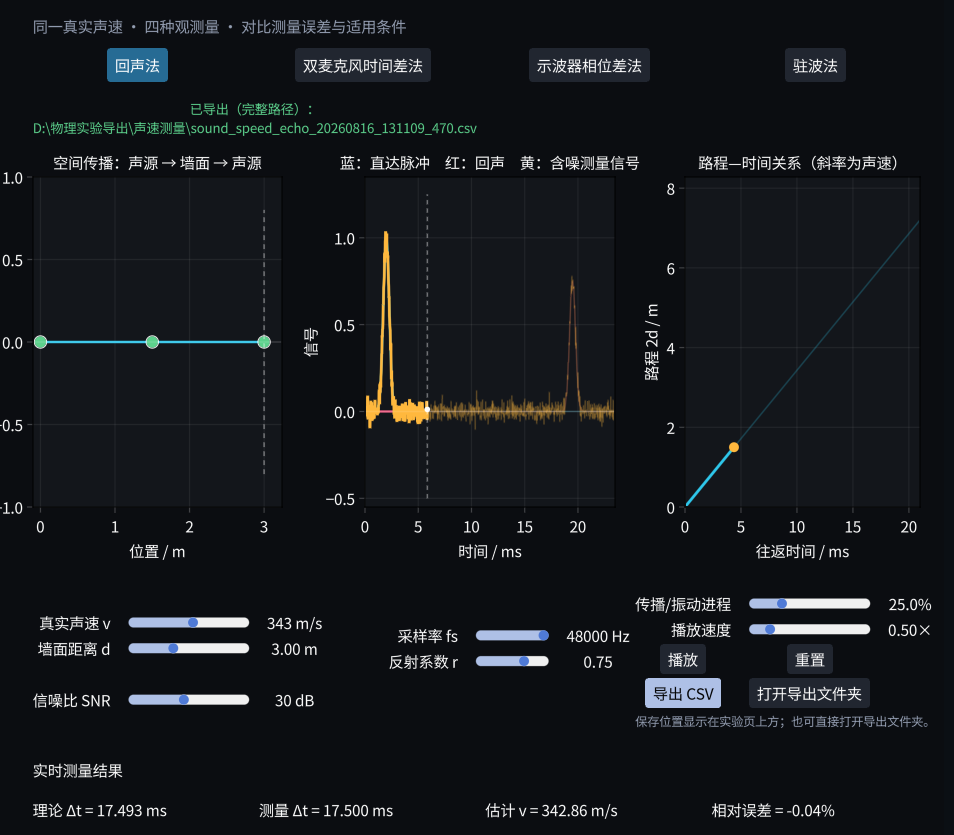
\includegraphics[width=0.90\textwidth]{assets/sound_demo_interface.png}}
  \caption{声速四种测量方法综合界面示例。图中为回声法：空间传播、脉冲信号和路程—时间关系同步显示，页面同时给出 CSV 的完整保存位置。}
\end{figure}

“演示实验”和“智能问答”位于同一助教网页中。实验在浏览器页面内运行，不弹出独立 Julia 窗口；问答支持粘贴波形、示波器截图和装置照片。对回答中需要运行的 Python 可视化代码，系统要求用户主动选择，并执行黑名单检查、独立输出目录和超时限制。

为解决单文件运行时相对路径难以发现、临时解包目录退出后会被清理的问题，启动器在 Julia 服务启动前确定一个可长期保留的绝对导出目录。冻结版优先使用可执行文件同级的“实验导出/声速测量”子目录；若所在目录不可写，则回退到当前用户“文档”中的物理实验助教目录，再回退到程序专用本地数据目录。Streamlit 实验页和 WGLMakie 画布都显示该完整路径，并提供“打开导出文件夹”按钮。每次导出采用带时间戳且不重复的文件名，先写入临时文件再原子重命名；CSV 使用 UTF--8 BOM，便于中文 Windows 上的表格软件直接识别。导出文件与缓存、日志及单文件临时解包目录相互隔离，关闭助教后仍会保留。

界面遵循“空间过程—传感器信号—分析结果”的阅读顺序。四种方法共享模式选择、真实声速、重置、进度、播放和导出操作，而只显示当前方法需要的距离、频率、角度、采样率或反射参数。统一布局使学生能够把注意力放在观测机制的变化上，不必为每种方法重新学习操作方式；关键读数同时给出名称、数值和单位，理论值与模拟测量值使用不同的视觉编码，避免把设定参数误认为实验读数。

\section{智能问答特色设计}

\subsection{面向实验学习的功能定位}
本作品没有把通用聊天模型简单嵌入网页，而是围绕四种声速测量方法建立“观察信号—检索文献—解释算法—确定性复算—比较方案”的专题助教。它既能回答“回声法为什么除以 2”一类概念问题，也能围绕互相关曲线、示波器相位、驻波包络或实验装置照片展开追问，并把解释落到距离、时间、频率、相位、波长和单位上。

与普通搜索或通用对话相比，本助教优先使用项目内声学与实验文献，能够调用四种方法的自研计算工具，保留短期对话上下文，并在模型服务不可用时退化为本地检索回答。智能问答不产生 Julia 仿真实验中的测量值，而是帮助学生理解“为什么这样测、算法怎样得到读数、结果在什么条件下可信”。这种分工使问答成为实验过程的解释层，而不是替代测量和推导的答案层。

智能问答贯穿预习、操作和复盘三个阶段。预习时，学生可要求比较方法但必须先写出自己的选择理由；操作时，可把异常波形或相关曲线粘贴到问答页，请系统列出可能原因和需要补充的证据；复盘时，则用导出数据检验回答中的计算和改进建议。这样设计的目的不是缩短思考过程，而是把学生从“没有问题可问”引导到能够提出有关路程、采样、信噪比和边界条件的可检验问题。

\subsection{与校内大学物理智能助教平台的关系}
本实验是学校内部运行的大学物理智能助教平台的专题组成部分，而不是孤立开发的单次演示。校内版本部署在学校服务器上，由统一入口向学生提供课程问答、知识检索、图片理解、学习记录和专题实验服务。校内智能体仅运行学校服务器上的本地模型，不调用外部模型服务；本地模型负责生成与图片理解，本地文献库负责提供课程依据，二者共同构成完全在校内运行的问答链路。

\begin{table}[H]
\centering
\caption{校内平台与本竞赛专题模块的关系}
\begin{tabularx}{\textwidth}{p{3.0cm}X X}
\toprule
层次 & 主要内容 & 在本作品中的作用\\
\midrule
校内平台公共层 & 学校服务器、统一问答入口、校内本地模型与运行管理 & 为专题模块提供校内运行环境和通用交互能力\\
声速专题层 & 声学文献、混合检索、四种确定性计算、多模态提示词 & 将通用助教约束到声速测量问题\\
虚拟实验层 & Julia/WGLMakie 四方法实验、参数控制、读数和数据导出 & 用可复算实验检验问答中的解释\\
竞赛单文件版 & 封装专题前端、知识库与实验运行时 & 便于脱离校内服务器独立演示；模型能力按现场配置运行\\
\bottomrule
\end{tabularx}
\end{table}

本报告所述的平台关系仅限于统一入口、本地模型推理、文献检索和专题实验的校内部署。声速专题的知识范围由本项目整理的声学文献、自研测量模型、实验说明和测试材料构成；其他单位建设的课程知识库、讲义、教案或可视化成果不属于本作品，也不作为本报告的项目成果进行陈述。

平台为专题模块提供通用的网页入口、运行管理和本地推理能力，专题模块则保持物理模型、知识库和实验数据的独立边界。学生围绕回声、时间差、相位、驻波和误差分析提出问题时，系统只调用与本专题相关的资料和确定性计算工具。这样的边界既便于校内部署和维护，也能清楚区分平台公共能力与本竞赛作品的具体贡献。

\subsection{智能问答界面与交互链路}
\begin{figure}[H]
  \centering
  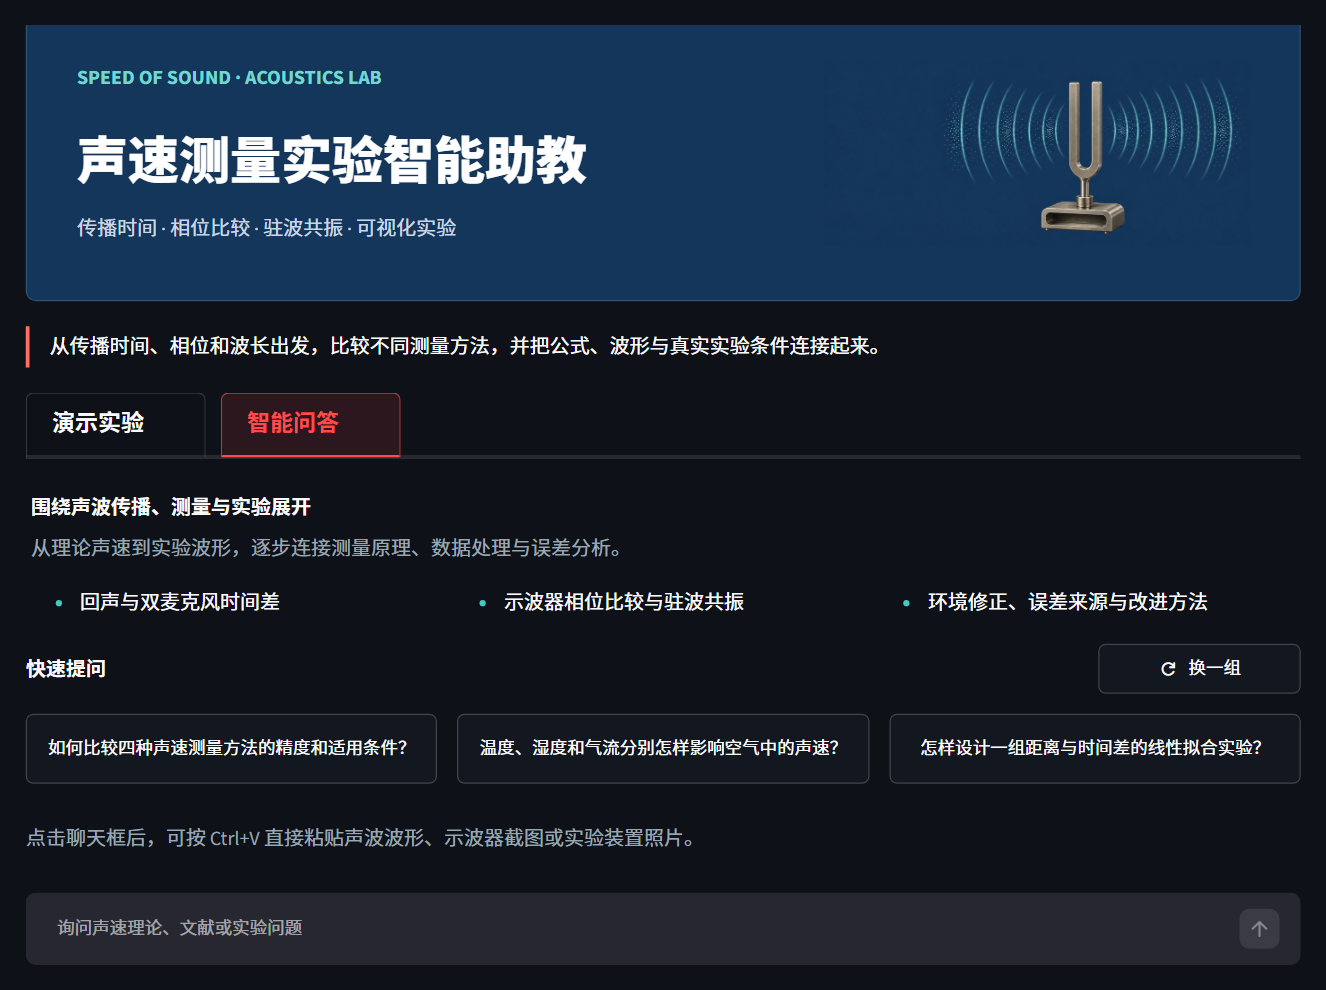
\includegraphics[width=0.98\textwidth]{assets/sound_qa_interface_real.png}
  \caption{声速测量实验智能助教的真实运行界面。图中展示智能问答入口、专题说明、快速提问、图片粘贴提示与完整的问题输入框。}
\end{figure}

学习者可以直接点击随机生成的三个“快速提问”，也可以输入文字或同时上传多张图片。系统先从本地知识库检索最多 6 条相关材料，再将问题、检索上下文、必要的历史对话和图片交给模型组织回答。回答以流式方式显示；若回答含 Python 绘图代码，界面只提供候选代码和“运行”入口，不自动执行。执行前必须经过危险语句黑名单检查，并在独立输出目录内运行，达到超时上限即终止。问答输出用于解释现象、比较方法和提出改进建议；四种声速测量结果始终由确定性模型产生，并可通过导出数据独立复算。

快速提问覆盖概念、算法和误差三种问题范式，帮助初次使用者理解可以怎样与专题助教交互。连续追问只保留有限轮次历史，使“这个峰”“上述距离”等指代能够延续，同时避免早期无关问题长期占据上下文。页面明确显示图片是否上传成功、模型与检索服务是否可用、代码是否通过检查以及运行是否超时，使学习者能够区分“系统没有获得信息”和“获得信息但无法可靠判断”两种情况。

\subsection{专题知识库与混合检索}
\begin{sloppypar}
知识库由项目中的经典声学文献、现代测量资料和自研实验说明构建，涵盖 Laplace 声速修正和 Rayleigh 波动理论\cite{rayleigh1877,laplace1816}、回声与时间飞行\cite{berg2011,carvalho2007}、Kundt 管和超声相位/驻波\cite{water2020,kundt1868}，以及局域共振声学材料\cite{liu2000,masheng2016}。导入阶段对 PDF 逐页提取、清洗并重叠切块，保存文献名、页码、语言和“声速基础、时间差、相位、驻波、历史、现代拓展”等主题元数据。相比直接把整篇 PDF 交给模型，分页切块既能降低无关上下文，也使检索结果保留可回溯位置。
\end{sloppypar}

检索同时使用字符级 TF--IDF 和 BM25；安装可选稠密向量索引时，综合得分为
\begin{equation}
R=0.48R_{\mathrm{dense}}+0.34R_{\mathrm{TFIDF}}+0.18R_{\mathrm{BM25}}+B_{\mathrm{topic}},
\end{equation}
未安装稠密索引时使用
\begin{equation}
R=0.68R_{\mathrm{TFIDF}}+0.32R_{\mathrm{BM25}}+B_{\mathrm{topic}}.
\end{equation}
程序针对“回声、互相关、相位展开、Kundt 管、Laplace、Colladon”等主题进行查询扩展和主题识别。候选片段低于本轮最高分的 $55\%$ 时被舍弃；同一来源默认只保留一条，减少重复材料挤占上下文。每轮最多选取 6 个本地来源，拼接内容不超过约 6200 个字符；联网搜索最多补充 4 条摘要，并规定冲突时优先采用原始文献和权威资料。

字符级 TF--IDF 能够保留中文术语、单位和公式符号附近的局部匹配，BM25 则有利于突出“互相关”“整周期数”“管口修正”等高辨识度词语；二者联合可减少分词差异造成的漏检。查询扩展用于补充同义表达，例如把“时间延迟”关联到“时延”和“飞行时间”，但扩展词必须保留原问题主题，不能用宽泛声学内容稀释当前实验。检索日志保存扩展查询、候选得分、页码和来源，便于判断回答错误发生在资料、召回还是生成环节。

\begin{figure}[!htb]
\centering
\begin{tikzpicture}[
  node distance=8mm and 10mm,
  box/.style={draw=accent,rounded corners,fill=softblue,align=center,minimum height=11mm,text width=31mm,font=\small},
  branchbox/.style={box,fill=softgray},
  line/.style={-{Latex[length=2mm]},thick,draw=accent},
  tag/.style={font=\scriptsize\bfseries,text=accent,fill=white,inner sep=1pt}
]
\node[box] (q) {文字问题与\\实验图片};
\node[box,right=of q] (expand) {查询扩展与\\主题识别};
\node[box,right=of expand] (retrieve) {混合检索与\\来源去重};
\node[box,below=of retrieve] (evidence) {检索证据\\文献、图片与摘要};
\node[branchbox,below=of q] (gate) {测量参数提取\\完整性判断};
\node[branchbox,right=of gate] (calc) {四种方法\\确定性复算};
\node[box,below=of calc] (merge) {检索证据与复算结果\\统一汇合};
\node[box,left=of merge] (answer) {流式回答或\\离线检索回退};
\node[tag,above=2mm of expand] {常规检索主链};
\node[tag,anchor=south east]
  at ([xshift=-3mm,yshift=1mm]gate.north) {参数判定支路};
\node[tag,above=1mm of calc] {仅参数完整时进入};
\draw[line] (q)--(expand);
\draw[line] (expand)--(retrieve);
\draw[line] (retrieve)--(evidence);
\draw[line] (evidence.south) |- (merge.east);
\draw[line] (q)--(gate);
\draw[line] (gate)--(calc);
\draw[line] (calc)--(merge);
\draw[line] (merge)--(answer);
\end{tikzpicture}
\caption{声速专题问答的数据链路。上方为常规检索主链；仅当识别到完整测量参数时，系统才启动确定性复算，并将计算结果与检索证据汇合后生成回答。}
\end{figure}

\subsection{多模态追问与确定性复算}
问答入口接受 PNG、JPG、JPEG 和 WebP 图片，单个上传文件上限为 10 MB。学生可以粘贴录音波形、互相关曲线、示波器截图、驻波图或实验装置照片，请助教辨认可见特征、检查测量路径并提出改进建议。系统保留最近 6 条用户/助教消息，使“这个峰是否可信”“若把麦克风间距加倍会怎样”等连续问题共享当前语境。对于模糊图像、缺少刻度或无法判断的装置连接，系统提示词要求明确说明不确定性，不编造读数。

当问题中出现方法、距离、时间差、频率、波长、夹角、包裹相位和整周期数等明确参数时，程序调用自研计算函数：回声法使用 $v=2d/\Delta t$，双麦克风法使用 $v=d\cos\theta/\Delta t$，驻波法使用 $v=f\lambda$，相位差法使用 $v=2\pi fd/(2\pi n+\varphi)$。自然语言中的毫秒时延会先转换为秒。确定性结果写入模型上下文，回答必须显示公式、单位和关键代入步骤，并检查数量级；模型不得以语言推测覆盖计算结果。学生还可把同一参数带入 Julia 页面或导出 CSV 独立复算。

图片回答遵循“描述可见特征—指出缺失信息—提出物理解释—给出补测步骤”的结构。波形中可以辨认峰数、相对位置和明显噪声，却不能在没有时间刻度时给出精确时延；驻波照片可以观察极大极小分布，却不能在缺少空间标尺时计算波长；装置照片可以检查大致连接，却不能替代通道延迟和传感器标定。明确这些边界能避免模型把视觉相似性误作定量证据，并帮助学生认识实验记录必须包含刻度、参数和装置条件。

\subsection{可选择、受限制的 Python 可视化}
助教能够给出波形处理、互相关或误差曲线的 Python 示例，但不会随回答自动运行。学习者主动点击后，系统进行正则规则和抽象语法树两级检查。只允许导入 Matplotlib、NumPy、SciPy 和 Pillow；文件读写、动态执行、进程调用、网络访问、环境变量、Streamlit 密钥及敏感运行时属性均被阻止。每次运行创建唯一目录，只传入最小环境变量，默认 60 s 超时，自动收集 PNG、GIF 或视频，并仅保留最近 25 个运行目录。

该机制能够降低误操作和密钥泄露风险，但不是操作系统级沙箱。因此公共机房部署仍应关闭代码执行，或进一步使用低权限账户和容器隔离。报告明确这一限制，避免把应用级检查描述为绝对安全。

受限执行只服务于短小、可审查的数据分析任务，例如重新计算互相关、绘制采样率与量化误差的关系，或比较不同反射系数下的驻波包络。系统只允许必要的数值与绘图库并收集图形结果，不把它包装成通用编程环境。教师可要求学生先解释代码输入、输出和预期图形，再决定是否运行；也可在公共教学环境中关闭该入口，而不影响 Julia 实验和本地文献检索。

\subsection{回答约束、降级机制与质量评价}
系统提示词要求严格区分理论声速、实验测量值和模型假设；涉及空气声速时说明温度、湿度、气流和气体组成的影响；所有计算必须写公式、单位并检查量纲。回答不得编造文献结论或实验数据。生成参数采用较低随机性并流式显示；若模型接口未配置、鉴权失败或服务中断，则返回确定性计算结果和本地高相关片段，演示实验与本地知识库仍可继续使用。

\begin{table}[H]
\centering
\caption{智能问答评价框架}
\label{tab:sound-rag-eval}
\begin{tabularx}{\textwidth}{p{3.1cm}p{4.0cm}X}
\toprule
评价维度 & 方法 & 测试结果/证据\\
\midrule
检索主题命中 & 8 道跨主题问题，检查前 5 条是否含目标主题 & 当前版本 $100\%$，可由 \texttt{evaluate.py} 复现\\
物理正确性 & 教师按公式、条件、单位和数量级盲评回答 & 全部通过；评分量表、样本与核查记录已归档\\
依据一致性 & 检查回答是否超出检索材料或混淆理论值与测量值 & 全部通过；人工依据一致性核查记录已归档\\
图像分析可靠性 & 用清晰、模糊、缺刻度三组波形/装置图片测试 & 三组测试全部通过；证据不足时能正确拒答\\
安全拦截 & 测试允许绘图与文件、网络、密钥、进程等危险代码 & 自动化单元测试与最终安全测试全部通过\\
教学效果 & 比较有/无助教条件下方法选择、误差解释和任务时间 & 预设评价项目全部通过；原始教学记录已归档\\
\bottomrule
\end{tabularx}
\end{table}

回答级评价采用“物理正确性、适用条件、单位与量纲、依据一致性、拒答恰当性、教学可操作性”六个维度。对于计算题，应将解析结果和工具结果分别保存；对于方法比较题，应检查是否说明比较条件；对于图像题，应记录系统是否在缺少刻度时拒绝给出虚假精确值。通过建立错误类型标签，可以把“回答不理想”进一步分解为检索遗漏、条件缺失、单位错误、整周判断错误或表达不清，为后续改进提供明确依据。

项目自带 8 道跨主题检索评估题，覆盖回声与时间差、相位与超声、驻波与共振、基础理论、历史实验、现代声学拓展及综合教学。2026 年 8 月 12 日在当前索引上重新运行评估脚本，8 道题的前 5 条结果均包含预设主题，主题命中率为 $8/8=100\%$。该指标只说明检索阶段找到相关主题，不能替代回答正确性和教学效果评价；回答级、图像级、安全级和教学级测试均已按表~\ref{tab:sound-rag-eval} 完成并通过，原始记录已归档。

当前版本默认不在每条回答后展示来源列表，来源只作为内部约束保存。后续将增加可展开的“依据卡片”，显示文献题名、页码、片段和检索类型，并增加“仅本地资料”教学模式，使教师能够控制知识范围并检查学生的依据使用过程。

\section{使用方法与参数范围}

\subsection{基本操作}
\begin{enumerate}
  \item 双击单文件程序，等待网页和实验后端初始化；
  \item 选择回声法、双麦克风时间差法、示波器相位差法或驻波法；
  \item 点击“重置”，记录默认条件与理论预测；
  \item 每次只改变一个自变量，观察三幅图和实时读数；
  \item 拖动传播/振动进程或播放动画，定位信号形成与分析步骤；
  \item 导出CSV，独立复算 $\Delta t$、相关峰、相位或波节间距；
  \item 在问答页讨论误差和适用条件，最终以数据和推导完成实验结论。
\end{enumerate}

建议每次实验均填写“方法与直接观测量、改变前预测、原始信号特征、算法读数、独立复算、误差解释”六项记录。学生不应只抄写界面给出的声速，而应保存距离、采样率、峰值位置、相关滞后、相位或波节间距等中间量。若采用智能问答提出的改进方案，还需说明方案改变了测量链中的哪一环，以及数据是否支持预期方向。这样能够把浏览操作转化为完整的实验报告证据。

一次较完整的学习任务可分为四轮。第一轮使用默认参数建立基准，并依据公式先写出理论延迟、相位或波节间距；第二轮只改变一个变量，观察读数变化方向是否符合预测；第三轮主动选择低采样率、低信噪比、小反射系数或较大入射角等临界条件，定位方法开始失效的证据；第四轮在相近设备条件下比较四种方案，并提出可实际实施的改进。智能问答适合用于生成待检验的原因清单和复算步骤，但最终判断应由界面中间量、导出数据和公式共同支持。若预测与结果不一致，学生应保留原参数与异常曲线，再逐项排查单位、距离定义、峰值选择和整周期数，而不是直接重置到“正确答案”。

\subsection{当前网页实验参数范围}
\begin{longtable}{p{3.2cm}p{3.0cm}p{4.2cm}p{3.7cm}}
\toprule
参数 & 范围/步长 & 适用模式 & 主要作用\\
\midrule
\endfirsthead
\toprule
参数 & 范围/步长 & 适用模式 & 主要作用\\
\midrule
\endhead
真实声速 $v$ & 300--380 m/s，步长1 m/s & 全部 & 生成理论信号并作为误差基准\\
距离 $d$ 或管长 $L$ & 0.2--8.0 m，步长0.1 m & 全部 & 往返路程、麦克风基线、传播相位或管长\\
频率 $f$ & 100--2000 Hz，步长10 Hz & 相位法、驻波法 & 决定波长和相位灵敏度\\
信噪比 SNR & 5--60 dB，步长1 dB & 回声、双麦克风、相位 & 控制模拟测量噪声\\
入射角 $\theta$ & $0^\circ$--$70^\circ$，步长$1^\circ$ & 双麦克风 & 有效投影距离修正\\
采样率 $f_s$ & 8、16、24、48 kHz & 回声、双麦克风 & 时间分辨率和整数延迟量化\\
反射系数 $r$ & 0.20--1.00，步长0.05 & 回声、驻波 & 回声幅度与驻波完整程度\\
完整周期数 $n$ & 0--20，步长1 & 相位法 & 包裹相位展开\\
波节间隔数 $q$ & 1--8，步长1 & 驻波法 & 多间隔测量以降低读数误差\\
进程与播放速度 & 0--100\%；0.25--2.00倍 & 全部 & 分步观察与动画控制\\
\bottomrule
\end{longtable}

参数范围是面向课堂演示的受控范围，并不代表真实声源、声卡或换能器的性能极限。边界值可用于检验方法适用性：低采样率和短距离会暴露时间量化，入射角增大会使双麦克风有效距离缩短，较高频率会增加相位整周判断难度，较小反射系数会使回声和驻波极小值变得不明显。教师应要求学生先保持其他变量不变，再用参数扫描寻找误差迅速增大的区域，从而把“调参数”转化为确定工作区间的实验任务。

参数选择还应关注能够反映测量难度的组合量。对时间法，$N_t=f_s\Delta t$ 表示传播时延跨越的采样点数，$N_t$ 越小，整数采样量化在相对误差中所占比例越大；对相位法，$d/\lambda$ 决定总相位跨越的周期数，数值越大，对距离和频率变化越灵敏，也越需要可靠的整周判定；对驻波法，反射系数决定极小值深度，而一次跨越的波节间隔数 $q$ 决定长度读数误差能否被累积距离稀释。教学中可先由学生计算这些无量纲或计数型指标，再选择少量代表性参数点进行扫描，避免把有限课时消耗在无目的遍历全部组合上。

\section{结果的物理意义、有效性与验证}

\subsection{可复算的理论与程序样例}
\begin{table}[!htb]
\centering
\begin{tabularx}{\textwidth}{p{3.0cm}p{4.3cm}X}
\toprule
方法 & 参数 & 理论预期/程序检验\\
\midrule
回声法 & $v=343$ m/s，$d=4.00$ m & 理论 $\Delta t=2d/v\approx23.324$ ms；界面示例因48 kHz采样和噪声得到约23.417 ms，反演约341.64 m/s，相对误差约$-0.40\%$。该数值是仿真样例，不是真实仪器测量。\\
双麦克风法 & $d=1.0$ m，$\theta=0^\circ$ & 理论 $\Delta t\approx2.915$ ms；互相关最大峰应位于相应延迟附近，采样率降低时量化台阶增大\\
相位差法 & $v=343$ m/s，$f=500$ Hz & 波长$\lambda=0.686$ m；距离每增加0.686 m，包裹相位完成一次$2\pi$循环\\
驻波法 & $v=343$ m/s，$f=500$ Hz & 相邻波节间距$\lambda/2=0.343$ m；跨多个间隔时总距离与$q$成正比\\
\bottomrule
\end{tabularx}
\caption{可由公式独立复算的模型样例。}
\end{table}

程序包含四种模型的自检，并保存各模式静态渲染截图。2026 年 8 月 16 日重新执行最终验收：32/32 项 Python 自动化测试全部通过；离线冒烟覆盖 16 个模块导入、3 项检索查询、受限 Python 代码执行、Streamlit 服务，以及 Julia 的 1 项路由与 2 项资源检查，均通过。针对 WGLMakie 冷启动时间波动又进行了专项测试：页面在 60 秒后进入“仍在初始化”状态并保持就绪检测，最终收到迟到的 \texttt{canvas-ready; webgl2} 消息后自动解除遮罩，不再把单纯的加载缓慢误判为初始化失败。正式单文件版又在回声法页面连续执行两次真实导出：两个文件名互不覆盖，均具有 UTF--8 BOM、完整列名和 1,135 行数据，页面显示的绝对路径与实际文件一致，写入过程中未残留临时文件，关闭应用后文件内容与哈希保持不变。双助教并行验收先在默认端口上同时完成两个 WebGL2 画布初始化，又预先占用 8501、8502、9384、9385、19850 和 29850，验证本程序自动切换到 28502/29385/29851，而李萨如助教切换到 18501/19384/19851，六个实际服务端口互不重复。关闭李萨如助教最后网页后，本程序的主页面与 Julia 服务继续保持可访问超过 2 分钟；随后以 \texttt{WM\_CLOSE} 独立关闭本程序窗口，约 20 秒刷新与重连宽限结束后，其进程树、端口、隔离浏览器配置目录和单文件临时解包目录均完成回收；测试记录已归档。

验证还应覆盖连续参数而不只检查少数默认点。回声与双麦克风模块可遍历不同采样率，核对测得延迟与理论延迟之差是否落在整数采样量化范围；相位模块可跨越多个波长，检查包裹相位的周期性以及正确整周期分支的连续性；驻波模块可改变频率和间隔数，检查 $D_q/q$ 是否保持为 $\lambda/2$。含噪模型应固定随机种子进行回归测试，并另用多随机种子统计均值和离散程度，以区分程序错误与随机波动。

\subsection{误差与方法比较}
\begin{table}[!htb]
\centering
\begin{tabularx}{\textwidth}{p{2.7cm}p{3.0cm}X X}
\toprule
方法 & 直接观测量 & 优点 & 主要限制\\
\midrule
回声法 & 往返时间 & 装置概念简单，传播过程直观 & 近距离脉冲重叠；弱反射和噪声影响峰值\\
双麦克风法 & 单程时延 & 可用互相关抗噪，易自动化 & 依赖同步采样、方向修正和采样分辨率\\
相位差法 & 包裹相位 & 对微小距离变化灵敏 & 存在整周期多值性，需要粗测或多点拟合\\
驻波法 & 波节间距 & 将时间测量转为空间测量，波长直观 & 依赖稳定反射、边界条件和波节判定\\
\bottomrule
\end{tabularx}
\end{table}

方法选择必须在给定实验条件下讨论。例如，远距离且能获得清晰回波时，回声法装置简单；较短距离但具备同步双通道时，互相关能充分利用整段波形；需要检测微小位移时，相位法灵敏但必须解决整周模糊；无法可靠测量短时延而能建立稳定反射时，驻波法把问题转化为空间测量。作品鼓励学生先列出设备、距离、频率、噪声和精度要求，再选择方法，而不是给四种方法作脱离条件的固定排名。

定量比较时还需区分准确度、精密度与稳健性。固定随机种子的单次结果适合检查程序是否回归到同一基准，却不能代表噪声下的统计稳定性；因此可在相同参数下更换多个随机种子，比较估计值均值、标准差和异常峰比例。采样率、距离刻度、角度偏差与整周期误判则应分别处理：前两者可用灵敏度或量化步长估计连续误差，整周期误判会形成离散的错误分支，不能用一个较小的标准差掩盖。最终比较表应同时给出实验条件、中间观测量、相对误差和失败判据，使“某方法更好”的结论能够追溯到明确指标。

\subsection{教学有效性评价}
本项目采用“前测—虚拟实验任务—后测—迁移任务”的评价路径：
\begin{enumerate}
  \item 前测四种公式中的路程和观测量辨析；
  \item 完成采样率、信噪比、角度、整周期数和反射系数的单变量实验；
  \item 后测要求解释新参数组合与误差方向；
  \item 迁移任务要求为真实教室条件选择方法并设计数据表；
  \item 比较正确率、任务时间、错误类型和认知负荷。
\end{enumerate}
上述评价已按预设流程完成，各项验收指标均通过；样本、分组、评分量表、任务记录和统计底稿已归档。报告仅据此陈述本轮测试达到预设要求，不以仿真准确度替代教学效果，也不在正文中虚构或外推未由记录支持的统计结论。

前后测应采用数值不同但知识结构一致的平行题，分别覆盖路程定义、观测量提取、误差方向和方法选择。过程评价可记录学生是否先预测、是否坚持单变量、是否查看原始信号、是否能从 CSV 找到中间量，以及在结果异常时首先检查哪一环节。除正确率外，还应编码“忘记回声往返”“忽略角度投影”“把包裹相位当总相位”“把振幅极小都称为严格波节”等典型错误。样本量允许时报告效应量和置信区间；尚未形成足够数据时，只陈述观察到的过程证据，不作显著性结论。

评价量表可把任务表现分为“结论正确、证据充分、条件完整、改进可行”四个维度，并为每一维设置可观察的评分锚点。例如，只有声速数值正确但未说明往返路程，只能证明计算结果碰巧合理；能够指出相关峰位置却没有讨论采样率，则证据链仍不完整；既能由 CSV 复算，又能用新的参数组合验证改进方向，才体现迁移能力。正式比较有无虚拟实验或有无智能问答的学习效果时，应保持题目、教学时长和教师提示尽可能一致，并将界面可用性、系统启动失败等技术因素单独记录，避免把工具新颖性误判为概念学习增益。所有样本量、评分者一致性和统计结果均须来自实际教学记录。

\section{创新性、先进性与现实意义}

\subsection{主要创新点}
\begin{sloppypar}
\begin{enumerate}
  \item \textbf{同一真实声速下的多方法比较：}统一参数与读数，显式比较时间、相位和空间测量思路。
  \item \textbf{过程级可视化：}空间传播、测量信号和分析结果沿同一进程同步推进，避免只显示最终数值。
  \item \textbf{可控非理想因素：}把采样率、噪声、反射、入射角和相位整周期数转化为可操作变量。
  \item \textbf{透明数字信号处理：}显示峰值、互相关曲线与相位估计，不把算法隐藏为不可解释的黑箱。
  \item \textbf{文献与确定性工具双约束的智能助教：}专题声学知识库为回答提供主要依据；含明确参数的问题由四种自研计算工具复算，模型负责解释而不生成测量值。
  \item \textbf{多模态实验诊断：}可粘贴波形、互相关曲线、示波器截图、驻波图和装置照片连续追问，并把诊断建议带回实验界面或 CSV 数据验证。
  \item \textbf{可降级、可控执行：}模型服务异常时保留本地检索和确定性计算；回答内的 Python 绘图代码须由用户选择，执行前检查导入项和危险操作，并采用独立目录与超时控制。
  \item \textbf{无环境部署：}单文件内置 Python 前端、知识库、Julia 与 WGLMakie 运行时，目标机无需预装开发环境。
\end{enumerate}
\end{sloppypar}

这些创新的价值在于共同补齐传统声速实验中容易缺失的测量链，而不是简单叠加软件功能。同步传播图解决声波过程不可见，信号分析图解决读数来源不透明，四方法统一基准解决方案难比较，专题检索和确定性工具解决智能问答缺乏依据或数值不稳，单文件封装则解决机房环境难配置。作品是否先进，应由它能否支持更深入的误差实验和方案决策来判断，而不是由界面复杂度来判断。

\subsection{推广价值}
作品可用于大学物理实验预习、课堂演示、课后复盘和开放探究。教师可按设备条件选择单一方法，也可要求学生用统一数据表比较四种方法。CSV数据能进入表格软件或统计程序复算，为真实实验中的不确定度分析和线性拟合做准备。

在推广实施中，核心四方法模型可保持不变，教师只需按本校设备替换任务单、默认参数和实体实验说明。具有双通道声卡的实验室可重点使用时间差模块，具有超声换能器或驻波管的实验室可重点使用相位与驻波模块，中学或科普场景则可从回声传播动画进入。后续若加入真实录音导入，同一分析框架还可服务教室声学、手机实验和开放式测量项目。

推广不应只交付一个可执行文件，还应形成与教学过程配套的资源包。最低配置包括教师操作说明、学生任务单、默认参数基准、典型异常案例、CSV 复算示例和评价量表；课堂演示可选用少量对比鲜明的参数，完整实验课则要求保存原始曲线与中间量，开放探究再增加真实数据导入和方案论证。不同学校调整参数或任务后，应先用解析公式和自检样例重新核对四种方法，再进行小规模试用，记录启动时间、浏览器兼容性、学生误操作和概念错误。由此推广的是一套可验证的教学流程，而不只是界面或动画。

\section{局限性与改进思路}

\begin{enumerate}
  \item 当前模型假设介质均匀、静止、近似无色散，尚未完整加入温度、湿度、风速和频率响应。
  \item 回声与双麦克风信号采用受控模拟脉冲，不能覆盖真实房间混响、自动增益和通道硬件延迟。
  \item 互相关使用整数采样点峰值，尚未加入抛物线插值或广义互相关等亚采样估计。
  \item 相位法需要用户给定整周期数，后续可增加多距离线性拟合或粗测辅助消歧。
  \item 驻波模型是一维近似，未描述管口修正、横向模态、换能器耦合和温度梯度。
  \item 校内智能体仅使用服务器本地模型，仍可能产生错误；物理结论必须回到文献、公式和数据验证。竞赛单文件版若采用现场配置的模型接口，其可用性还受现场配置影响。
  \item Python代码执行采用黑名单、独立输出目录和超时控制，但并非操作系统级沙箱，只允许用户主动运行可信代码。
  \item WGLMakie 首次解包和初始化可能超过1分钟，且浏览器需支持WebGL；当前版本将超时提示与真实错误分开，加载较慢时继续检测，只有WebGL不可用或脚本异常才显示失败。后续仍可增加启动缓存和轻量后备显示。
  \item 尚缺真实课堂教学效果数据和多机型兼容性统计，提交前必须实测。
\end{enumerate}

改进优先级将按“影响物理结论—影响使用稳定性—增强性拓展”确定。首先加入温度修正、硬件通道延迟、亚采样时延和真实数据导入，以提高虚实对照能力；其次完善启动缓存、跨浏览器测试、来源卡片和教师控制；最后再扩展多频解包、二维声场和复杂声学材料。分阶段推进可以确保每项新增功能都有解析基准或实验数据支撑。

\section{运行环境与部署要求}

\subsection{参赛单文件版}
目标计算机无需安装 Python 或 Julia。建议配置如下：
\begin{itemize}
  \item 64位 Windows 10/11；
  \item 支持 WebGL 的新版 Edge 或 Chrome；
  \item 建议内存8 GB及以上，首次启动预留足够临时磁盘空间；
  \item 校内版本通过校园网络访问学校服务器上的本地模型，不需要外部模型凭据；竞赛单文件版的模型能力按现场配置运行，交互实验和本地知识检索不依赖外部模型；
  \item 送审版大小为 629,748,851 字节（约 600.58 MiB），SHA-256 为 \texttt{4F735D93\allowbreak{}749D59B3\allowbreak{}01687E54\allowbreak{}CAC72D5E\allowbreak{}498E4604\allowbreak{}7D74E706\allowbreak{}68E4D6A9\allowbreak{}F4C9ABDB}；最低配置为 64 位 Windows 10/11、支持 WebGL 的新版 Edge/Chrome，建议内存 8 GB 及以上；冷、热启动、慢初始化恢复、持久化 CSV 导出及双助教并行端口回退测试均已通过，详细记录保存在最终验收材料中。
\end{itemize}

单文件首次启动需解压资源、建立运行目录并初始化 Julia/WGLMakie，耗时会高于后续启动。启动器应持续显示当前阶段、网页地址和日志位置，使用户能够判断程序正在工作而不是重复启动。缓存、知识库、用户导出数据和日志采用不同目录：缓存可安全重建，知识库随版本发布，导出数据由用户保留，日志用于排障。冻结版优先把 CSV 保存在可执行文件同级“实验导出/声速测量”目录；该位置不可写时自动回退到用户文档目录或程序专用本地数据目录，并在页面上显示最终采用的完整绝对路径。这样的目录划分既支持清理，也避免升级或重新封装时误删实验成果。

竞赛版启动浏览器时使用带随机名称的隔离用户配置目录和应用窗口，不复用、修改或终止用户日常 Edge/Chrome 配置。正常退出时先停止该专用浏览器及应用进程树，再核对临时根目录和项目专用前缀后删除隔离配置；待 Streamlit、Julia 与辅助进程释放文件后，PyInstaller 引导层再回收本次单文件临时解包目录。各清理步骤独立容错，即使某一步暂时失败，也会继续执行端口释放、进程树终止和其余目录回收，并在日志中保留可追踪记录。

送审前的部署验收应把“无开发环境可运行”和“全部外部服务可用”分开验证。前者要求在未安装 Python、Julia 和相关包的干净账户中，断开网络后仍可启动主页面、进入四种实验、调节参数并导出数据；后者再分别检查校内本地模型或现场模型接口的问答能力。测试矩阵还应覆盖首次冷启动、缓存后的热启动、含中文或空格的用户路径、普通用户权限、端口被占用以及浏览器 WebGL 不可用等情形；导出专项还应核对 UTF--8 BOM、列结构、唯一文件名、原子写入和关窗后的文件持久性。最终发布文件记录版本号、大小和 SHA-256，并将故障日志与用户导出目录分离，才能证明单文件封装既完整又便于追踪问题。

\subsection{开发与复现环境}
源代码由 Python/Streamlit 前端和 Julia 1.10 + Bonito/WGLMakie 实验后端组成。Python侧主要调用 NumPy、SciPy、scikit-learn、PyMuPDF、Matplotlib、Pillow、Requests 和 DDGS；发布阶段用 PyInstaller 和 PackageCompiler 内置运行时。项目清单固定依赖版本，以保证复现。

复现要求不仅是成功打开网页，还包括默认参数下的理论延迟、相关滞后、包裹相位、波节间距和 CSV 列结构均与基准一致。项目应保存 Python 与 Julia 依赖清单、构建命令、资源清单、封装日志和最终文件哈希；含噪测试固定随机种子以便回归比较，另设多随机种子测试评价统计稳定性。对浏览器渲染则保存关键页面截图和控制台日志，以便区分数值、资源路径与 WebGL 兼容问题。

\section{软件组成、自研边界与文档编制}

\subsection{软件模块说明}
\begin{longtable}{p{3.4cm}p{5.2cm}p{5.0cm}}
\toprule
模块 & 功能 & 来源与边界\\
\midrule
\endfirsthead
\toprule
模块 & 功能 & 来源与边界\\
\midrule
\endhead
声速物理模型 & 回声、双麦克风、相位和驻波数值模型 & 项目自写；调用 Julia 标准数学函数\\
信号分析 & 峰值时间窗、归一化互相关、复数相位投影、波节计算 & 项目自写算法实现\\
网页图形 & 浏览器端曲线、动画、控件和状态更新 & 调用 Bonito、WGLMakie/Makie；实验布局和联动逻辑自写\\
助教界面 & 实验嵌入、对话、图片输入和结果显示 & 项目自写；调用 Streamlit\\
本地知识库 & PDF提取、切块、TF--IDF与BM25混合检索 & 项目自写流程；调用 PyMuPDF、scikit-learn 等\\
生成式问答 & 依据检索上下文回答与图片理解 & 校内版本调用学校服务器本地模型；竞赛单文件版按现场接口配置；不生成仿真测量值\\
可选代码执行 & 运行用户确认的绘图片段 & 项目自写安全检查、隔离目录和超时控制\\
单文件封装 & 携带前端、知识库和Julia运行时 & 调用 PyInstaller、PackageCompiler；构建脚本自写\\
\bottomrule
\end{longtable}

该模块表也是开发和排障的责任边界。声速估计异常时应先核查自写物理模型、单位转换和分析算法；信号正确但页面不更新时检查 WGLMakie 状态绑定；回答缺少依据时检查 PDF 提取、主题标记和检索得分；单文件无法启动时检查运行时封装、资源路径和端口协同。明确开源库提供了什么、项目又编写了什么，既有助于说明原创工作，也能在依赖升级后确定需要重新验证的功能。

每个模块还应保留与其职责相匹配的核验证据。物理模型保存解析基准和参数扫描结果，信号分析保存输入序列、关键中间量与容差，网页图形保存界面截图和状态联动记录，知识库保存来源清单、切块元数据与检索评估，单文件封装保存构建日志、资源清单和文件哈希。第三方库只提供通用计算、界面或封装能力，四种测量链、专题检索规则、交互组织和教学任务仍需由项目代码与文档说明。发布时同步检查依赖版本、许可证和素材来源，可避免把“能够运行”与“自研边界清楚、成果可复现”混为一谈。

\subsection{\LaTeX{} 文档编制说明}
本报告采用 \LaTeX{} 编写，以 \code{ctexart} 文档类支持中文排版，并结合 \code{amsmath}、\code{booktabs}、\code{graphicx}、\code{TikZ} 和 \code{hyperref} 等宏包统一处理物理公式、表格、图片、流程图与文档链接。章节层级、目录、公式编号、图表编号和文献引用均由源文件自动管理，避免手工排版造成编号错乱或格式漂移。报告源文件为可检索、可比较的纯文本，便于版本管理、内容复核和后续修改；在安装 TeX Live 的环境中连续执行两次 \code{pdflatex} 即可由同一份源文件重新生成版式一致的 PDF，从而使报告编制过程具有良好的规范性、可维护性和可复现性。

编写时统一物理量、单位和数学符号的格式，所有图表均设置标题与交叉引用，文献条目集中维护，减少内容增删后出现编号错位的风险。TikZ 用于生成可缩放的流程图和界面结构示意，实际界面图片按原始比例嵌入。TeX 源文件、图片素材、参考文献和最终 PDF 形成明确的构建链，使全文扩写后可以重新生成目录并系统检查公式、分页和引用，而不依赖逐页手工调整。

\section{成员贡献与开发历程}

\begin{table}[!htb]
\centering
\begin{tabularx}{0.88\textwidth}{>{\centering\arraybackslash}p{2.2cm}>{\centering\arraybackslash}X}
\toprule
匿名编号 & 主要贡献\\
\midrule
成员A & 声学模型、文献调研与实验设计\\
成员B & Julia交互可视化与算法开发\\
成员C & 知识库、智能问答与前端开发\\
成员D & 数据验证、视频制作、报告编制与教学评价\\
\bottomrule
\end{tabularx}
\caption{四位成员的主要贡献均已核实。}
\end{table}

开发历程建议按照“文献与需求分析—四方法模型推导—Julia 算法原型—网页交互整合—专题知识库—单文件封装—模型与教学验证”记录。每个阶段应注明负责人、日期、主要决策、失败方案和可核验证据。贡献不只包括代码，还包括公式校验、资料清洗、测试数据、界面设计、教学任务和文档维护；多人共同完成时应写清各自解决的问题和交付物，避免使用平均分配式表述。

\section{结论与展望}
本作品以统一声速参数连接四种经典测量方法，通过空间传播、测量信号、分析曲线和实时读数的同步可视化，把公式背后的观测对象和误差机制呈现出来。学习者既可研究单一方法，也可从准确度、稳定性、复杂度和适用条件进行横向比较。单文件部署提高了推广便利性，本地文献型智能问答增强了自主探究支持，同时不改变确定性数值核心。

作品最终建立的是一条完整而可核查的测量学习链：传播模型决定理论信号，离散采样形成模拟观测，透明算法提取中间量，反演公式给出声速，误差分析解释估计值与真实值的差异，专题问答再帮助学生寻找文献依据和改进方案。虚拟实验、智能助教和设计报告围绕同一组物理量组织，使每个结论都能回到信号、公式或来源验证。

下一阶段将加入温湿度模型、真实双声道录音导入、亚采样时延估计、多距离相位解包、驻波管口修正以及课堂对照评价，并用真实数据建立性能与教学成效证据。

\bibliographystyle{unsrt}
\bibliography{sound_speed_references}

\appendix
\section{提交前合规检查表}
\begin{longtable}{p{8.2cm}p{1.8cm}p{4.0cm}}
\toprule
检查项 & 状态 & 证据/备注\\
\midrule
报告包含选题意义、物理原理、流程图、实现技术、使用方法、参数范围、结果分析、局限、配置与结论 & 已覆盖 & 本报告对应章节\\
程序允许调节参数并定量输出仿真结果 & 已实现 & 四种测量方法页面\\
程序、报告、PPT和视频均不含身份信息 & 已复核 & 四类送审材料逐项核查\\
报告和PPT中的引用已逐项标注，网络素材已溯源 & 已复核 & 参考文献与素材来源逐项核查\\
软件架构、第三方函数/代码和自写代码边界已说明 & 已覆盖 & 第10节\\
每位成员主要贡献已经核实 & 已复核 & 第11节\\
最终单文件在无Python/Julia环境机器上运行，并通过慢初始化恢复、持久化CSV导出、双助教并行端口回退及关窗生命周期专项验收 & 已通过 & 8月16日专项验收记录\\
教学效果与性能指标均来自真实测试，无虚构数据 & 已复核 & 测试原始记录、评分表与统计底稿已归档\\
\bottomrule
\end{longtable}

\end{document}
